\begin{frame}[Generate]{Erasing virtual methods, CRTP} 
\begin{itemize}
\item Curiously Recurring Template Pattern.
\item \cite{eli}
\end{itemize}
\end{frame}

\begin{frame}[fragile]{CRTP, run time polymorphism}
\inputminted[mathescape,
           linenos,
           numbersep=5pt,
           frame=lines,
           bgcolor=White,
           fontsize=\tiny,
           linenos,
           framesep=2mm]{c++}
           {/Users/lalanne/MyCode/GitHubProjects/MetaTalk/src/code/run_complex_pol_mine_1.cpp} 
\end{frame}

\begin{frame}[fragile]{CRTP, run time polymorphism}
\inputminted[mathescape,
           linenos,
           numbersep=5pt,
           frame=lines,
           bgcolor=White,
           fontsize=\scriptsize,
           linenos,
           framesep=2mm]{c++}
           {/Users/lalanne/MyCode/GitHubProjects/MetaTalk/src/code/run_complex_pol_mine_2.cpp} 
\end{frame}

\begin{frame}[fragile]{CRTP, compile time polymorphism}
\inputminted[mathescape,
           linenos,
           numbersep=5pt,
           frame=lines,
           bgcolor=White,
           fontsize=\tiny,
           linenos,
           framesep=2mm]{c++}
           {/Users/lalanne/MyCode/GitHubProjects/MetaTalk/src/code/comp_complex_pol_mine_1.cpp} 
\end{frame}

\begin{frame}[fragile]{CRTP, compile time polymorphism}
\inputminted[mathescape,
           linenos,
           numbersep=5pt,
           frame=lines,
           bgcolor=White,
           fontsize=\scriptsize,
           linenos,
           framesep=2mm]{c++}
           {/Users/lalanne/MyCode/GitHubProjects/MetaTalk/src/code/comp_complex_pol_mine_2.cpp} 
\end{frame}

\begin{frame}[fragile]{CRTP, compile time polymorphism}
\inputminted[mathescape,
           linenos,
           numbersep=5pt,
           frame=lines,
           bgcolor=White,
           fontsize=\scriptsize,
           linenos,
           framesep=2mm]{c++}
           {/Users/lalanne/MyCode/GitHubProjects/MetaTalk/src/code/comp_complex_pol_mine_3.cpp} 
\end{frame}


\begin{frame}[fragile]{CRTP, compile time polymorphism}
    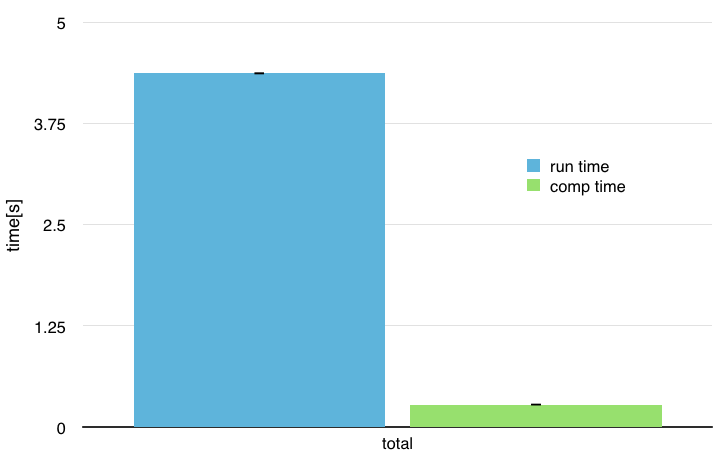
\includegraphics[scale=0.3]{/Users/lalanne/MyCode/GitHubProjects/MetaTalk/figures/crt.png}
\end{frame}

\begin{frame}[fragile]{Logical CPU balance}
\vspace{20mm}
\begin{figure}
\begin{tikzpicture}[font=\footnotesize,xshift=-25mm,yshift=-17mm]
\begin{axis}[
scale only axis,
xmin=  1,xmax=240,
minor tick num =4,
every tick/.style={thick},
xlabel=hw threads, ylabel=time/s,
width=0.55\textwidth,
]
\addplot +[blue,thick] table[x index=0, y index=  1] {figures/vtune.dat};
\end{axis}
\end{tikzpicture}
\end{figure}
\vspace{20mm}
\par{15 MPI processes each 4 threads running on Xeon Phi}
\end{frame}

